\begin{figure}[t]
	\centering
	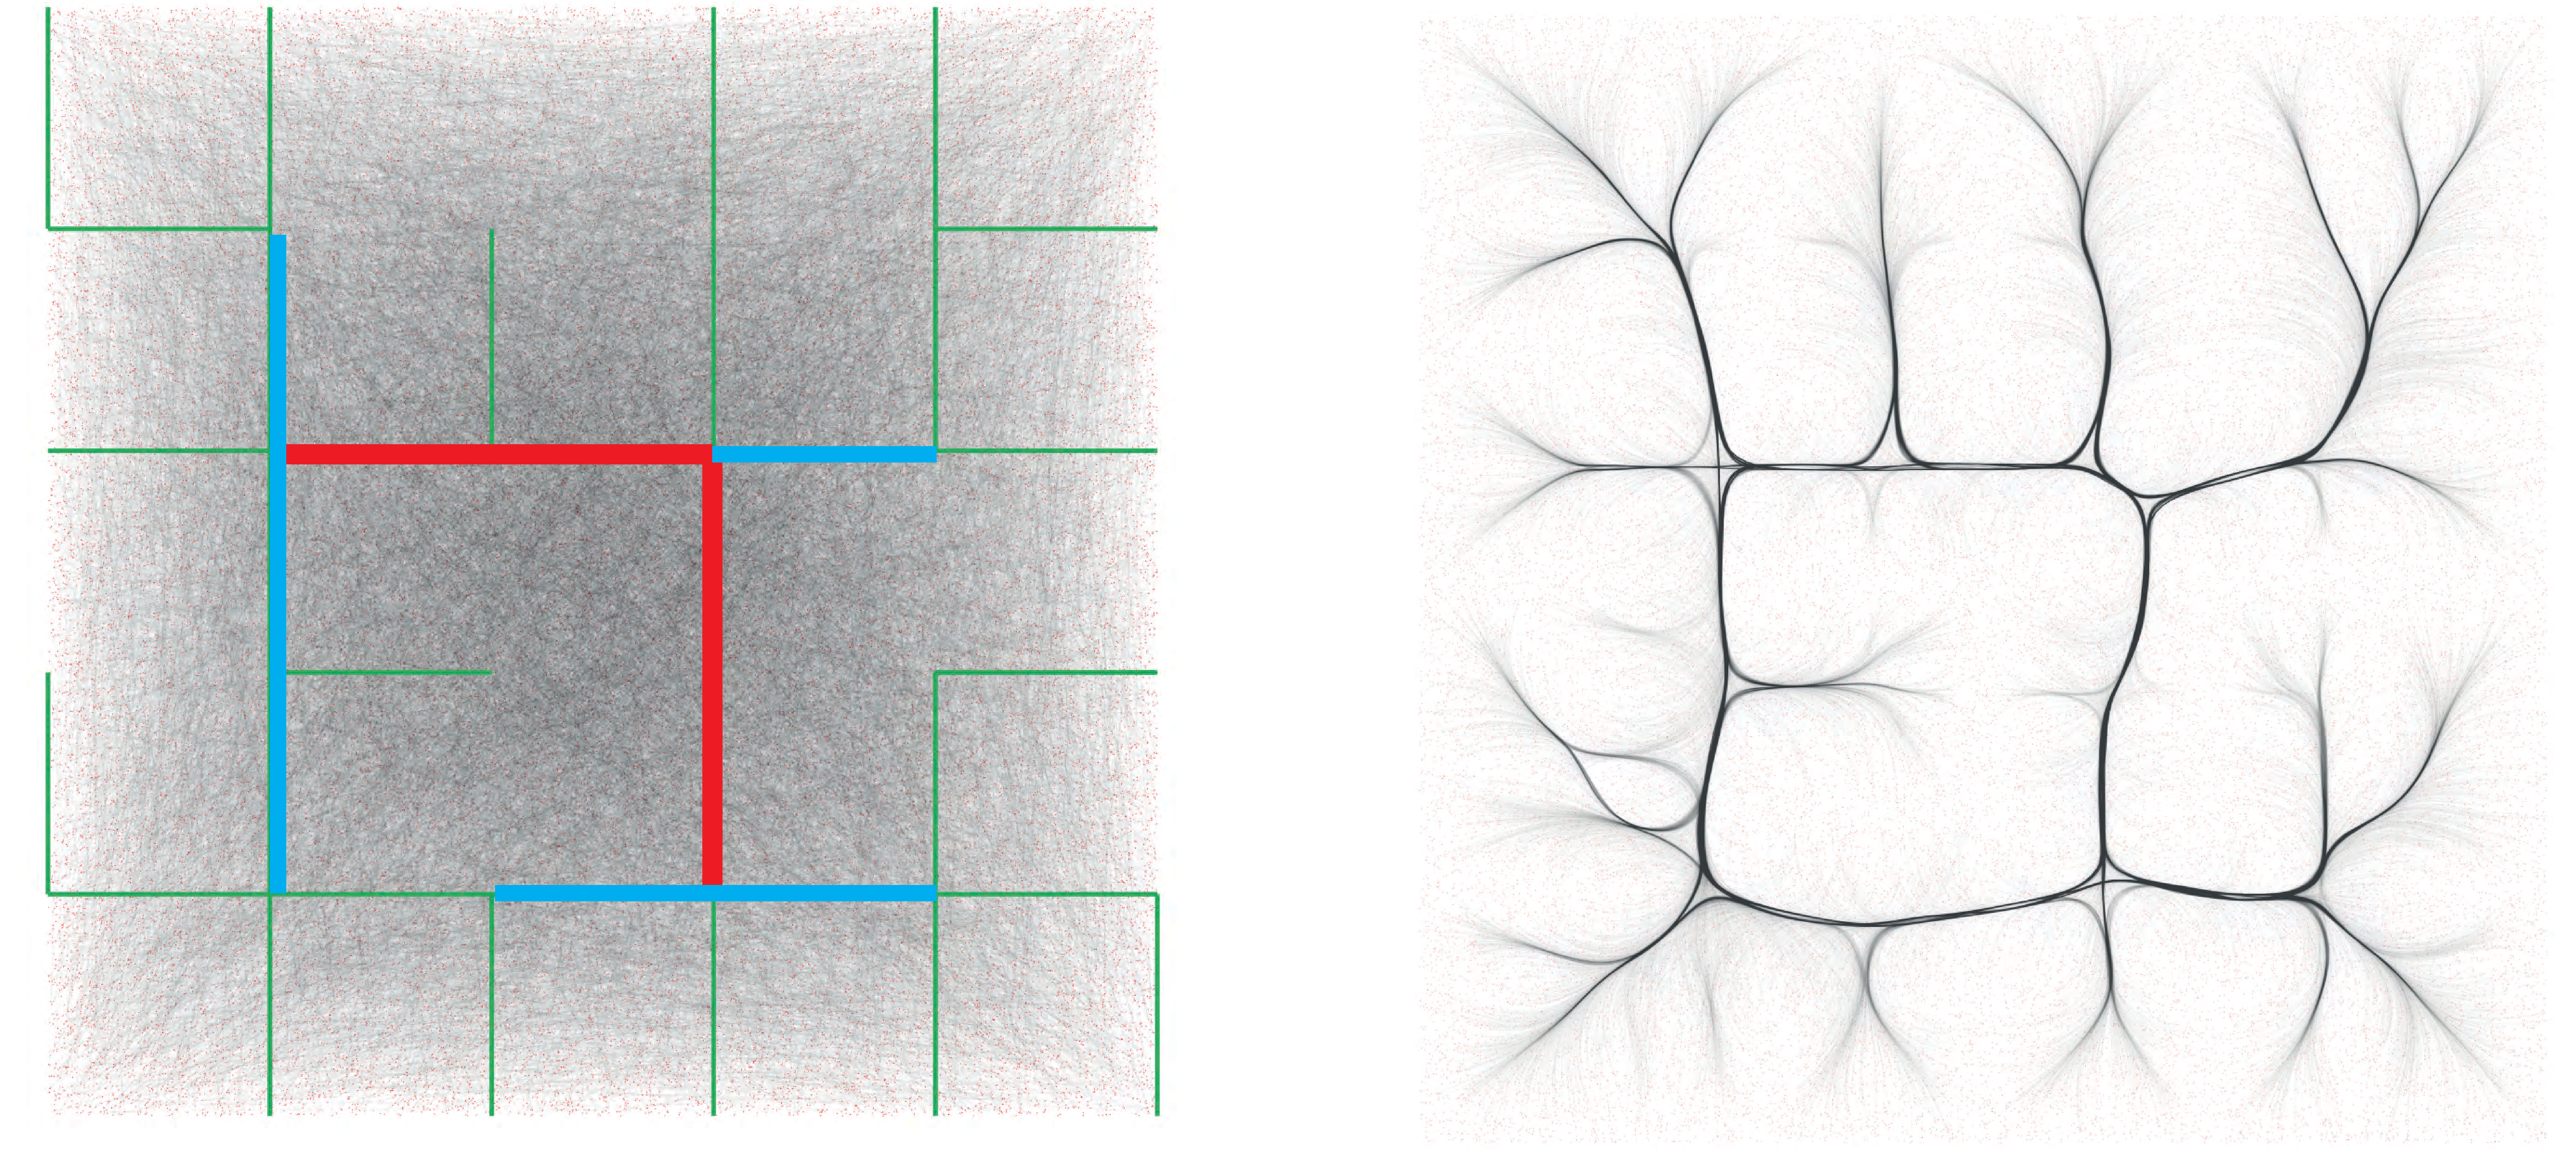
\includegraphics[width=0.49\textwidth]{figure/edgebundling/fig7_hierar/artifical}
	\vspace{-6mm}
	\caption{
		Left: raw 100K artificial OD trails on a hierarchical road network.
		Right: RAEB bundling result with $p_{ra}$ set to 2.
		}
	\label{fig:hier}
	\vspace{-5mm}
\end{figure}

\section{Applications}
This section presents applications of RAEB on artificial OD trails, and real-world taxi data in New York and Shenzhen.
We show advancements of RAEB over KDEEB.

\begin{figure*}[t]
	\centering
	\includegraphics[width=0.995\textwidth]{figure/edgebundling/fig8_study2/NYC}
	\vspace{-2mm}
	\caption{Density maps of NYC taxi trips:
	(a) shortest paths mapped onto the road network, 
	(b) KDEEB bundles with kernel size $p_r$ = 60,
	(c) KDEEB bundles with $p_r$ = 21,
	and (d) our RAEB bundles with $p_r$ = 21.}
	\label{fig:nyc_visual}
	\vspace{-4mm}
\end{figure*}

\begin{figure}[t]
	\centering
	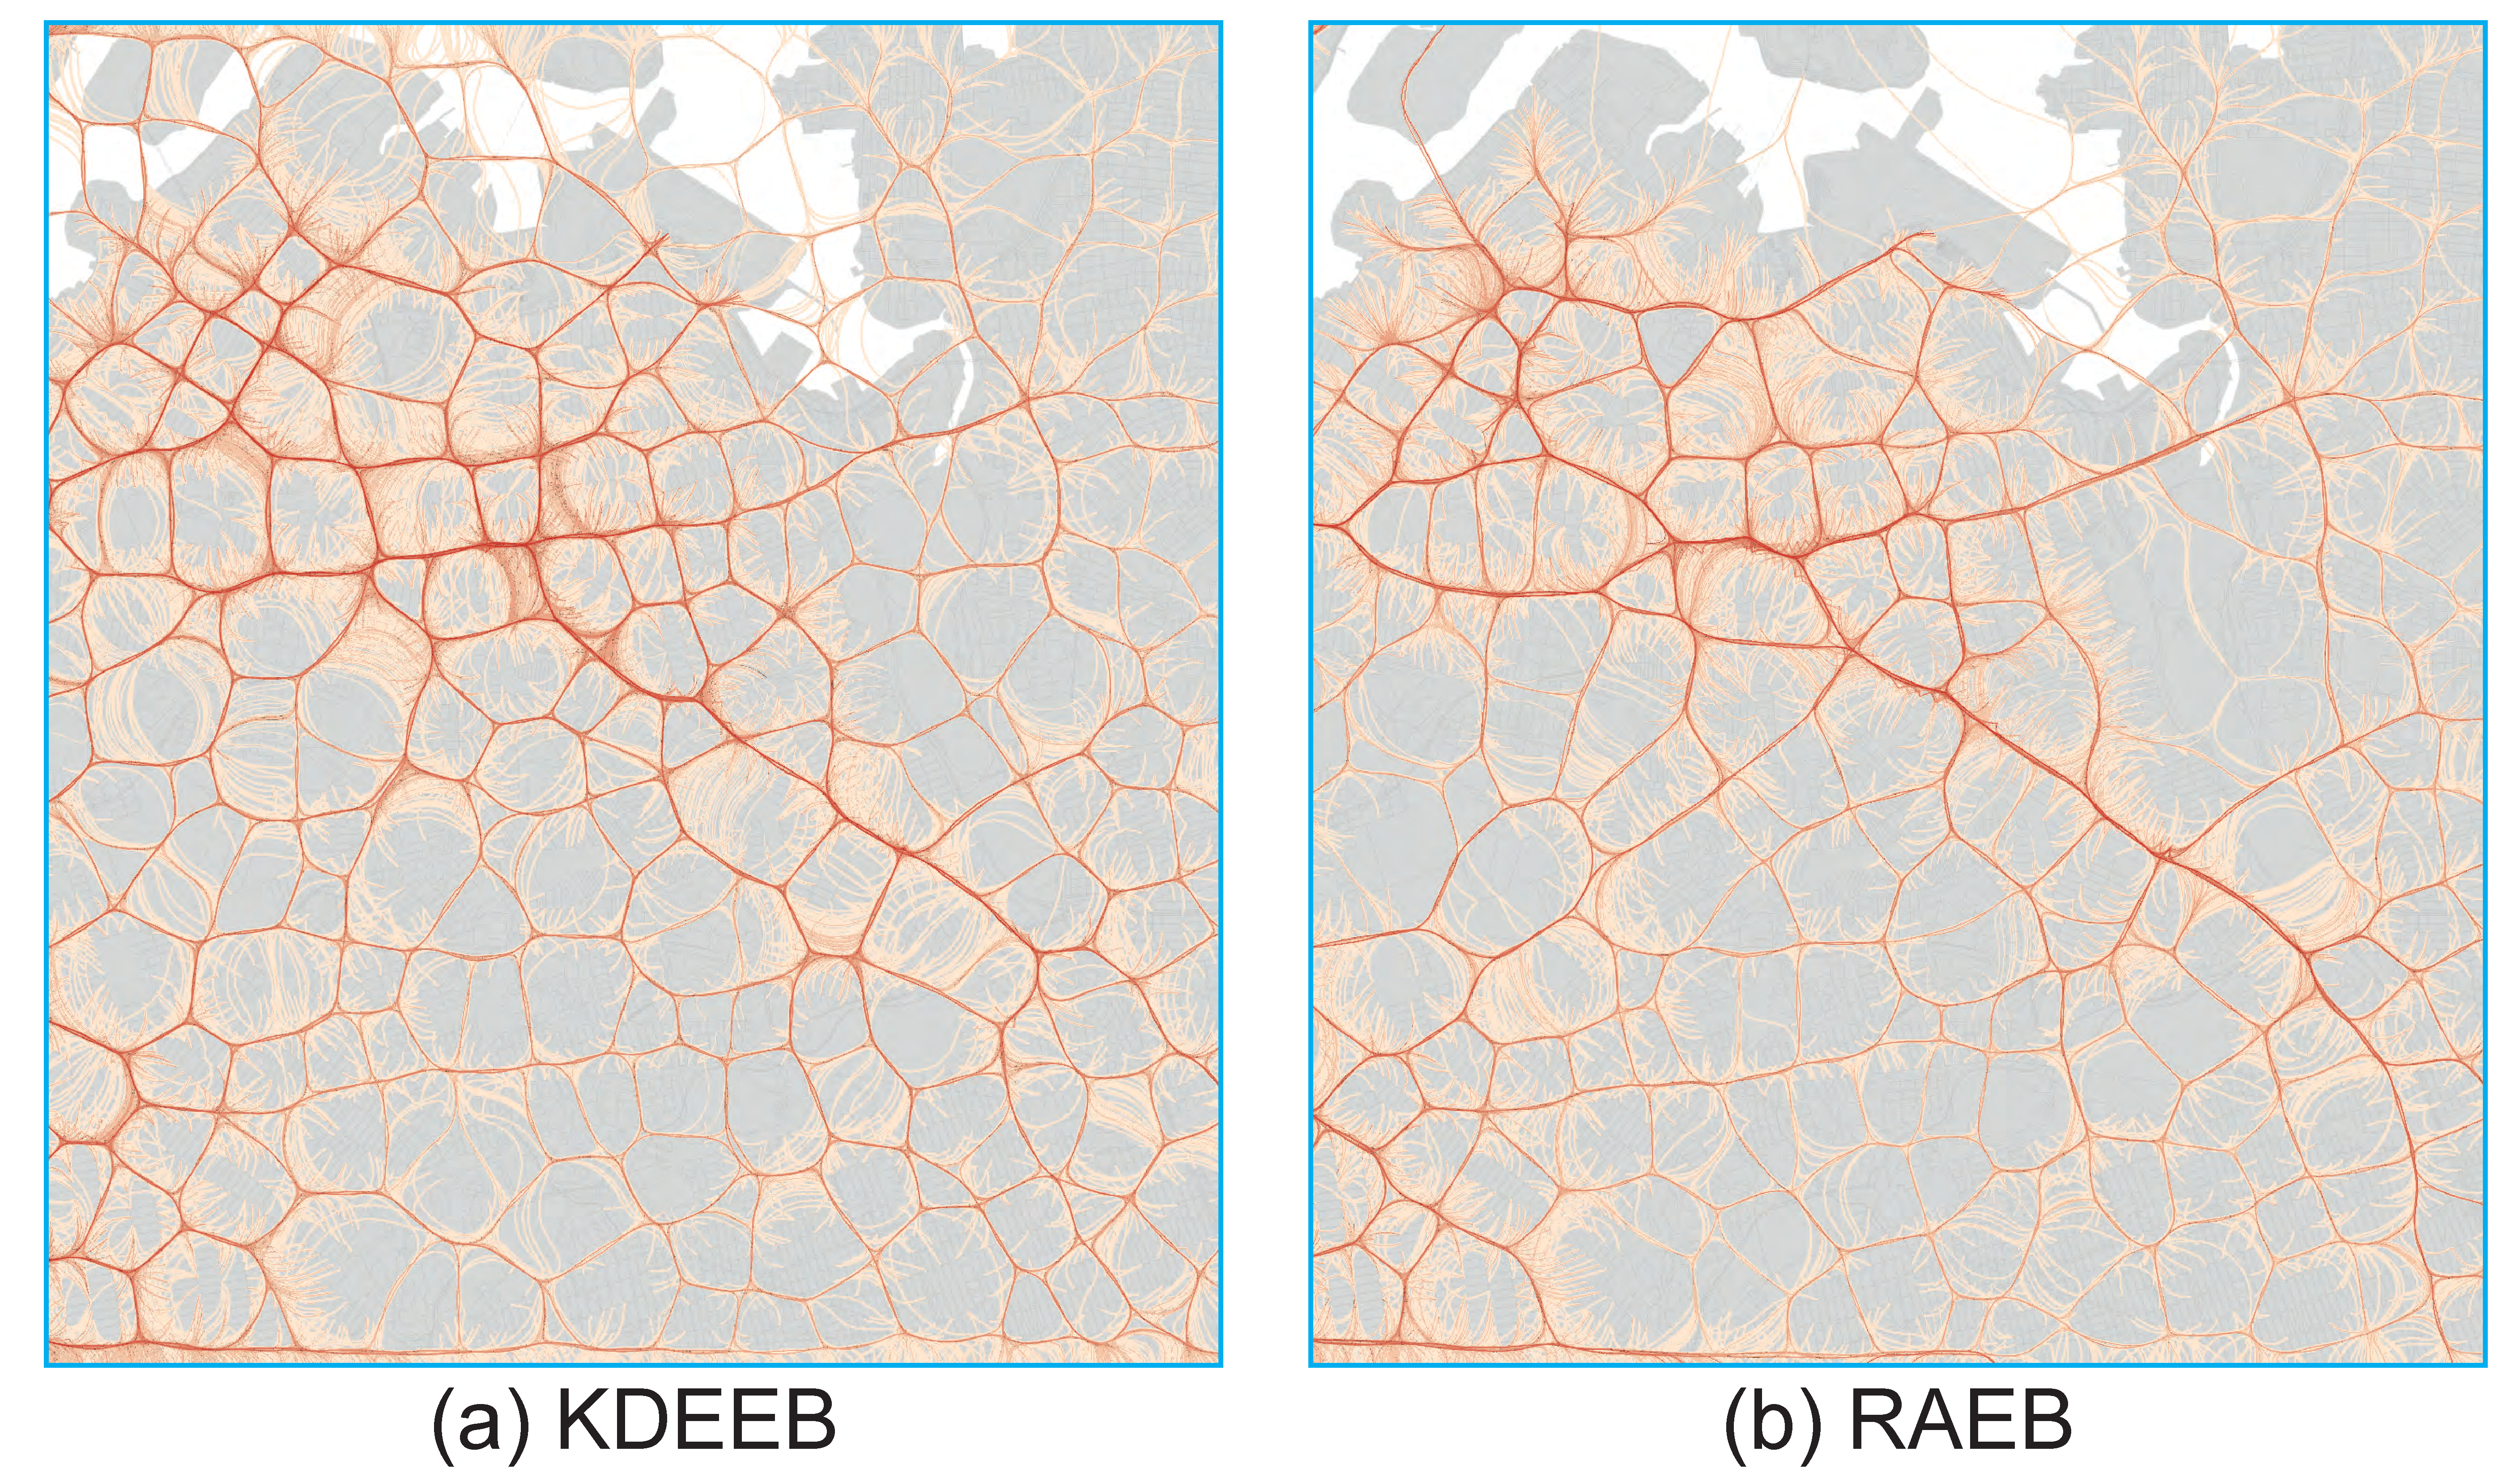
\includegraphics[width=0.45\textwidth]{figure/edgebundling/fig9_study2-2/NYC-zoom}
	\vspace{-3mm}
	\caption{Fine scale density maps of NYC taxi trips in Queens zone generated by (a) KDEEB, and (b) RAEB.}
	\label{fig:nyc-zoom}
	\vspace{-4mm}
\end{figure}

%%%%%%%%%%%%%%%%%%%%%%%%%%%%%%%%%%%%%%%%%%%%%%%%%%%%%%%%%%%%%%%%%%%%%%%%%%%%%%%%%%%%
\subsection{Artificial OD Trails}
\label{ssec:study1}

Our first example uses a random graph with 100K OD trails, and $5 \times 5$ grid and hierarchical reference graphs to simulate conventional road networks.
Raw OD trials and corresponding road networks are shown in the leftmost figures of Figure~\ref{fig:grid} and Figure~\ref{fig:hier}.
The OD trails are first mapped to underlying road networks using shortest path algorithm, and then both road networks are divided into three hierarchies that are colored in red, blue and green, receptively.
In the last, we apply RAEB on the OD trails, with all graph drawing sizes set to 1280$\times$1280 and initial kernel sizes $p_r$ set to 60.

In advance of KDEEB, RAEB allows to preserve route awareness by controlling parameter $p_{ra}$.
To evaluate the effects of $p_{ra}$, we set $p_{ra}$ to 0 - 3, and apply RAEB to OD trails on the grid road network as shown in the leftmost figure of Figure~\ref{fig:grid}.
The results are shown in Figure~\ref{fig:grid} (a) - (d).
In (a), $p_{ra}$ is set to 0, i.e., no route awareness will be preserved.
In this case, RAEB should be equivalent to KDEEB with other parameters the same.
The proof is demonstrated in (a), which shows smooth bundles similar to those in the original KDEEB~\cite{hurter2012graph}.
To preserve level 1 routes, we set $p_{ra}$ to 1, and the result is shown in (b).
As expected, OD trails around the red lines are bundled together with bundles following red lines, while other OD trails are bundled with bundles spreading arbitrarily in the graph drawing.
More route awareness can be preserved as we increase $p_{ra}$ to 2 and 3, as shown in Figure~\ref{fig:grid} (c) \& (d).

More importantly, route awareness $p_{ra}$ can be used to preserve topology of underlying road network.
Figure~\ref{fig:hier} (right) shows bundling result of RAEB applied to OD trails on a hierarchical road network that is shown in Figure~\ref{fig:hier}(left).
Here, $p_{ra}$ is set to 2, such that to preserve both the red and blue lines.
It is clear that the resulting bundles follow the lines, making it easy to trace OD trails.
In contrast, KDEEB will generate the same result with that in Figure~\ref{fig:grid}(a), as the underlying road network information is not used.

\begin{figure*}[t]
	\centering
	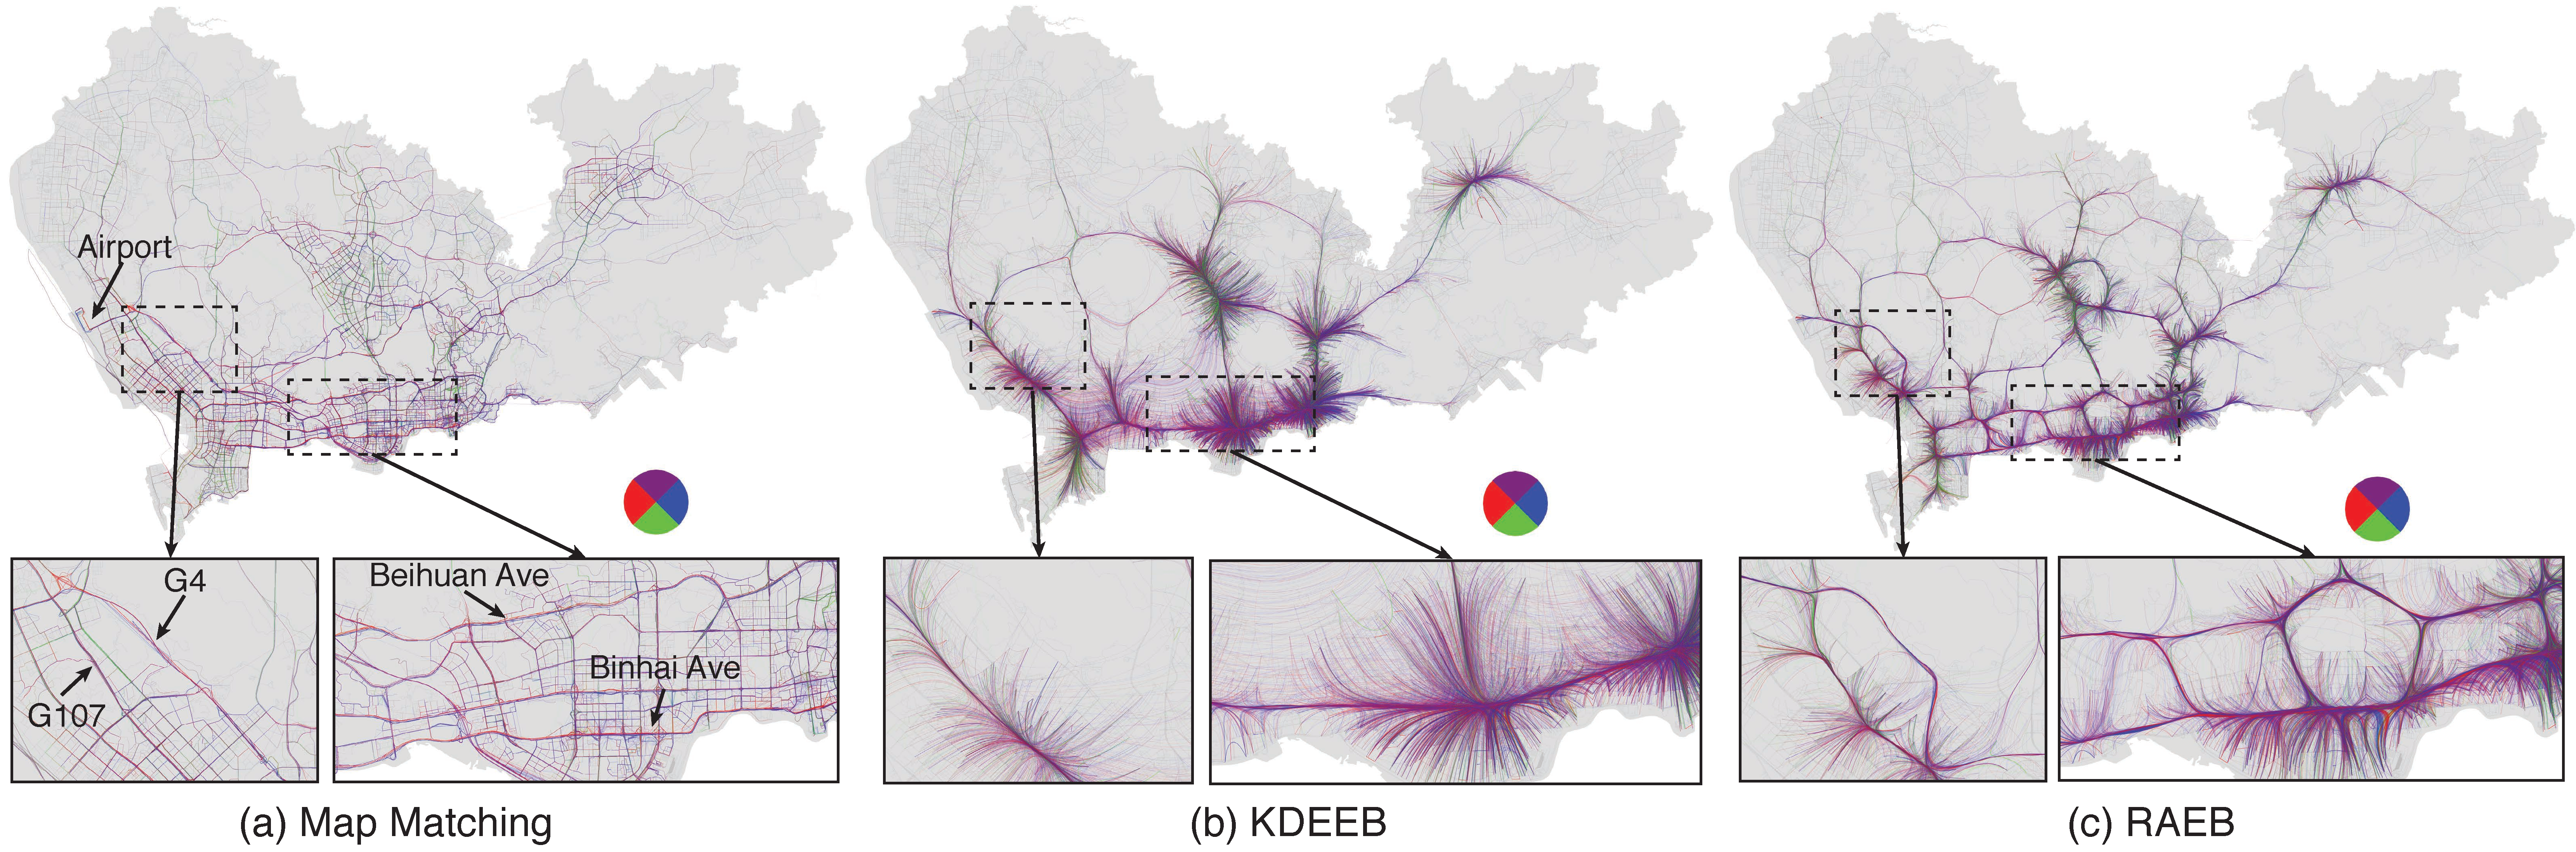
\includegraphics[width=0.995\textwidth]{figure/edgebundling/fig10_study3/shenzhen}
	\vspace{-2mm}
	\caption{
	Density maps of Shenzhen taxi trips: (a) raw GPS records are mapped onto road network, (b) KDEEB bundles trips on close aterial roads together, while (c) RAEB preserves these roads. All lines are colored according to the OD directions.
	}
	\label{fig:shenzhen}
	\vspace{-4mm}
\end{figure*}

%%%%%%%%%%%%%%%%%%%%%%%%%%%%%%%%%%%%%%%%%%%%%%%%%%%%%%%%%%%%%%%%%%%%%%%%%%%%%%%%%%%%
\subsection{New York Taxi Trips}
\label{ssec:study2}

In reality, a road network is usually much more complex, and OD trails are more dynamic than the artificial ones.
In this experiment, we further compare RAEB with KDEEB using results generated from New York taxi trips.

The road network employed in this study is extracted from OpenStreetMap (OSM) within the boundary of Manhattan, Brooklyn, Queens, and Bronx zones, where most origins and destinations are located.
The raw network consists of 133,154 nodes, 166,122 edges, and it is simplified to 97,336 routes.
The OD trails studied in this experiment are 100K taxi trips extracted from one-month trip records.
The original records consist of various attributes for each trip, including vendor id, pickup \& dropoff times and positions, and fare amount, etc.
We use the pickup \& dropoff positions, and map it onto the road network using shortest path algorithm.
Figure~\ref{fig:nyc_visual}(a) presents a density map of the mapped taxi trips.

Figure~\ref{fig:nyc_visual}(b - d) show bundling results generated by KDEEB and RAEB, with graph drawing sizes set to 1080 $\times$ 1440.
The experiment is started with KDEEB recommended settings of kernel size $p_r$ = 60 (about 5\% of graph drawing size) and $p_n$ = 10.
Figure~\ref{fig:nyc_visual}(b) shows the bundling result, which clearly presents several main bundles.
The bundles reveal primary traffic movements over the whole city.
Yet in other ways, the results are heavily bundled, missing details of road network topology.
To show more details, we measure initial kernel size considering both graph drawing and geometric property of road network as described in Section~\ref{ssec:kernel_size}.
$p_r$ is reduced to 21.
Figure~\ref{fig:nyc_visual}(c) shows the corresponding KDEEB bundling results.
More bundles are formed, in line with arterial roads in New York.
However, there are many bundles lying by non-existing roads, as those shown in the highlighted region in-between Manhattan and Brooklyn.
This illustration can cause wrong impression of bridges connecting the zones.
Figure~\ref{fig:nyc_visual}(d) shows results generated by RAEB, with $p_r$ = 21 and route awareness $p_{ra}$ = 1.
The undesirable bundles are removed by our method.

Visualization of urban traffic should support multi-scale exploration $-$ an important characteristic for movement data visualization.
In the context of this work, a good edge bundling algorithm should provide smooth transitions of bundling results at different scales.
We further evaluate multi-scale exploration by zooming into the blue region in Queens zone as in Figure~\ref{fig:nyc_visual}(c) \& (d), and applying KDEEB and RAEB on the OD trails.
The fine scale bundling results are presented in Figure~\ref{fig:nyc-zoom}(a) \& (b), respectively.
More bundles are generated by both methods, as the same effect when zooming into maps.
However, it is difficult to visually match bundles in Figure~\ref{fig:nyc_visual}(c) with those in Figure~\ref{fig:nyc-zoom}(a).
In comparison, bundles in Figure~\ref{fig:nyc_visual}(d) can be more easily identified in Figure~\ref{fig:nyc-zoom}(d).

%%%%%%%%%%%%%%%%%%%%%%%%%%%%%%%%%%%%%%%%%%%%%%%%%%%%%%%%%%%%%%%%%%%%%%%%%%%%%%%%%%%%
\subsection{Shenzhen Taxi Trips}
\label{ssec:study3}

We further evaluate the performance of RAEB using taxi trips in Shenzhen, with road network extracted from OSM.
In total, there are 161K nodes and 177K edges, and the edges are simplified to 51K routes.
The OD trails are one-week taxi trip records.
Unlike New York taxi records with only origin and destination positions, Shenzhen's data contain a sequence of GPS positions recorded in every 20 seconds.
We clean and extract in total 50K taxi trips from the records.
The trips are further mapped onto the road network using ST-matching algorithm~\cite{lou_2009_map}.

Figure~\ref{fig:shenzhen}(a) presents a graph of the map matching results in the size of 2160$\times$1280.
The lines of a trip are colored according to direction from the trip's origin to destination.
The graph shows that most taxi trips are recorded in the southern region of Shenzhen, which borders on Hong Kong and is more developed than other regions.
The unevenly distributed taxi trips make it improper to use kernel size $p_r$ recommended by KDEEB, which is over 100 as 5\% of the graph drawing size.
Instead, our method suggests $p_r$ = 26, considering the road network topology as well.

Using this setting of $p_r$, both KDEEB and RAEB reaches stable states at iteration 8.
Figure~\ref{fig:shenzhen}(b) \& (c) show the corresponding results, respectively.
Both methods create smooth bundles in line with arterial roads in Shenzhen, indicating $p_r$ measured by our method is preferable.
Besides, nearly the same bundles are generated in regions other than south part, except that RAEB's result shows more details.
More dissimilar results are shown in the highlighted areas.
Expressways G4 and G107 lead traffic to Shenzhen airport in the left region, while Beihuan and Binhai avenues holds main traffic in the right one.
KDEEB merges OD trails passing these roads, while our method splits the bundles.
In short, RAEB generates results more similar to real-world scenarios.